\section{Addition}

\begin{outcome}
  \begin{enumerate}
  \item Compute sums and differences of vectors algebraically and
    geometrically.
  \item Use the laws of vector addition to prove equalities between
    vector expressions.
  \end{enumerate}
\end{outcome}

Addition of vectors in $\R^n$ is defined as follows.

\begin{definition}{Addition of vectors in $\R^n$}{vector-addition}
For vectors $\vect{u}=\begin{mymatrix}{c}
u_{1} \\
\vdots \\
u_{n}
\end{mymatrix},\; \vect{v}= \begin{mymatrix}{c}
v_{1} \\
\vdots \\
v_{n}
\end{mymatrix} \in \R^{n}$, the
sum\index{vector!addition}\index{addition!of vectors}
$\vect{u}+\vect{v}\in \R^{n}$ is defined by
\begin{equation*}
\vect{u}+\vect{v} = \begin{mymatrix}{c}
u_{1} \\
\vdots \\
u_{n}
\end{mymatrix} +  \begin{mymatrix}{c}
v_{1} \\
\vdots \\
v_{n}
\end{mymatrix}
= \begin{mymatrix}{c}
u_{1}+v_{1} \\
\vdots \\
u_{n}+v_{n}
\end{mymatrix}.
\end{equation*}
\end{definition}

To add vectors, we simply add corresponding components. Therefore, in
order to add vectors, they must be the same size.  For example,
$\mat{ 1, 2, 3 }^T + \mat{ 4, 5, 6 }^T = \mat{ 1+4, 2+5, 3+6 }^T =
\mat{ 5, 7, 9 }^T$.

The geometric significance of vector addition in $\R^n$ is given in
the following proposition.

\begin{proposition}{Geometry of vector addition}{geometry-of-vector-addition}
  Let $\vect{u}$ and $\vect{v}$ be two vectors in $\R^n$. Slide
  $\vect{v}$ so that the tail of $\vect{v}$ is on the tip of
  $\vect{u}$. Then draw the arrow which goes from the tail of
  $\vect{u}$ to the tip of $\vect{v}$.  This arrow represents the
  vector $\vect{u}+\vect{v}$.

  \begin{center}
    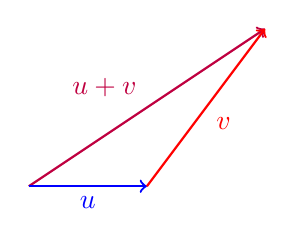
\begin{tikzpicture}[scale=2]
      \draw[->, thick, purple](0,0) -- node[above left]{$\vect{u}+\vect{v}$}(1.5,1);
      \draw[->, thick, blue](0,0) -- node[below]{$\vect{u}$} (0.75,0);
      \draw[->, thick, red](0.75,0) -- node[below right]{$\vect{v}$} (1.5,1);
    \end{tikzpicture}
  \end{center}
\end{proposition}

\begin{example}{Commutative law}{comm-law-geo}
  Let $\vect{u}$ and $\vect{v}$ be two vectors. Using the geometry of
  vector addition, explain why $\vect{u}+\vect{v} = \vect{v} + \vect{u}$.
\end{example}

\begin{solution}
  In the following diagram, the vectors $\vect{u}$ and $\vect{v}$ form
  a parallelogram. Therefore, whether we line up the tail of
  $\vect{u}$ with the tip of $\vect{v}$ or vice versa, we obtain the
  same vector, which is both $\vect{u}+\vect{v}$ and
  $\vect{v}+\vect{u}$.
\begin{center}
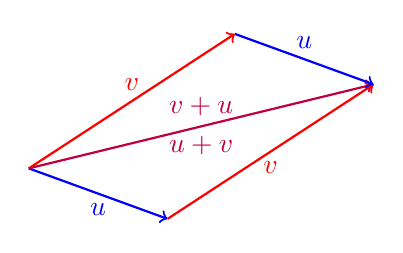
\begin{tikzpicture}[scale=2.5,rotate=-20]
\draw[->, thick, purple](0,0) -- node[above]{$\vect{v}+\vect{u}$}
     node[below]{$\vect{u}+\vect{v}$} (1.5,1);
\draw[->, thick, blue](0,0) -- node[below]{$\vect{u}$} (0.75,0);
\draw[->, thick, red](0.75,0) -- node[below]{$\vect{v}$} (1.5,1);
\draw[->, thick, blue](0.75,1) -- node[above]{$\vect{u}$} (1.5,1);
\draw[->, thick, red](0,0) -- node[above]{$\vect{v}$} (0.75,1);
\end{tikzpicture}
\end{center}
\end{solution}

\begin{definition}{Negative}{vector-negative}
  The \textbf{negative}\index{vector!negative}%
  \index{negative!of a vector} of a vector
  $\vect{u}=\begin{mymatrix}{c}
    u_{1} \\
    \vdots \\
    u_{n}
  \end{mymatrix}\in\R^{n}$ is defined by 
  $-\vect{u} = \begin{mymatrix}{c}
    -u_{1} \\
    \vdots \\
    -u_{n}
  \end{mymatrix}$.
\end{definition}

Geometrically, the vector $-\vect{u}$ has the same magnitude as
$\vect{u}$, but the opposite direction.
\begin{center}
  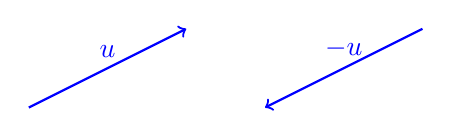
\begin{tikzpicture}
    \draw[->, thick, blue](0,0) -- node[above]{$\vect{u}$} +(2,1);
    \draw[->, thick, blue](5,1) -- node[above]{$-\vect{u}$} +(-2,-1);
  \end{tikzpicture}
\end{center}

To define the \textbf{subtraction}\index{vector!subtraction}%
\index{subtraction!of vectors} of two vectors, we simply regard
$\vect{u}-\vect{v}$ as an abbreviation for
$\vect{u} + \tup{-\vect{v}}$, exactly as we do with real
numbers. Algebraically, this just amounts to componentwise
subtraction:
\begin{equation*}
  \begin{mymatrix}{c}
u_{1} \\
\vdots \\
u_{n}
\end{mymatrix} - \begin{mymatrix}{c}
v_{1} \\
\vdots \\
v_{n}
\end{mymatrix}
= \begin{mymatrix}{c}
u_{1}-v_{1} \\
\vdots \\
u_{n}-v_{n}
\end{mymatrix}.
\end{equation*}

The following example illustrates how to subtract vectors
geometrically.

\begin{example}{Graphing vector addition}{graphing-vector-addition}
Consider the following picture of vectors $\vect{u}$ and $\vect{v}$.

\begin{center}
\begin{tikzpicture}[scale=2]
\draw[->, thick, blue] (0,0) -- node[above]{$\vect{u}$} (2,1);
\draw[->, thick, red] (4,1) -- node[above]{$\vect{v}$} (5,0.5);
\end{tikzpicture}
\end{center}

Sketch a picture of $\vect{u}+\vect{v}$ and $\vect{u}-\vect{v}$.
\end{example}

\begin{solution}
We will first sketch $\vect{u}+\vect{v}$. Begin by drawing $\vect{u}$
and then at the point of $\vect{u}$, place the tail of $\vect{v}$ as
shown. Then $\vect{u}+\vect{v}$ is the vector which results from
drawing a vector from the tail of $\vect{u}$ to the tip of $\vect{v}$.

\begin{center}
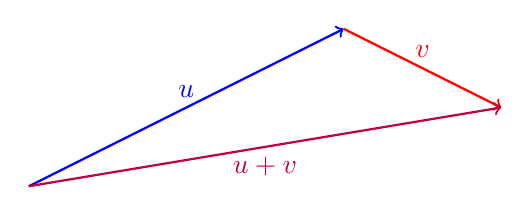
\begin{tikzpicture}[scale=2]
\draw[->, thick, blue] (0,0) -- node[above]{$\vect{u}$} (2,1);
\draw[->, thick, red] (2,1) -- node[above]{$\vect{v}$} (3,0.5);
\draw[->, thick, purple](0,0) -- node[below]{$\vect{u}+\vect{v}$} (3,0.5);
\end{tikzpicture}
\end{center}

Next consider $\vect{u}-\vect{v}$. This means $\vect{u}+\tup{-\vect{v}
}$. From the above geometric description of vector addition, $-\vect{v}$ 
is the vector which has the same length but which points in the
opposite direction to $\vect{v}$. Here is a picture of $-\vect{v}$ 

\begin{center}
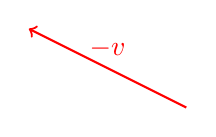
\begin{tikzpicture}[scale=2]
\draw[<-, thick, red] (4,1) -- node[above]{$-\vect{v}$} (5,0.5);
\end{tikzpicture}
\end{center}

The following picture fully represents $\vect{u}-\vect{v}$:

\begin{center}
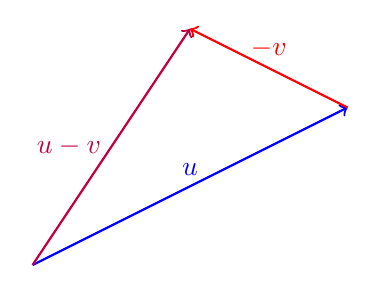
\begin{tikzpicture}[scale=2]
\draw[->, thick, blue](0,0) -- node[above]{$\vect{u}$} (2,1);
\draw[<-, thick, red] (1,1.5) -- node[above]{$-\vect{v}$} (2,1);
\draw[->, thick, purple](0,0) -- node[left]{$\vect{u}-\vect{v}$}(1,1.5);
\end{tikzpicture}
\end{center}

Given any two vectors $\vect{u}$ and $\vect{v}$ one can create a
parallelogram with sides these vectors and diagonals
$\vect{u}+\vect{v}$ and $\vect{v}-\vect{u}$:

\begin{center}
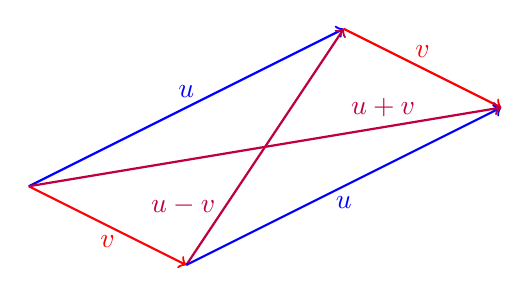
\begin{tikzpicture}[scale=2]
\draw[->, thick, blue](-1,0.5) -- node[above]{$\vect{u}$} (1,1.5);
\draw[->, thick, red] (1,1.5) -- node[above]{$\vect{v}$} (2,1);
\draw[->, thick, purple](0,0) -- node[left, near start]{$\vect{u}-\vect{v}$}(1,1.5);
\draw[->, thick, blue](0,0) -- node[below]{$\vect{u}$} (2,1);
\draw[->, thick, red](-1,0.5) -- node[below]{$\vect{v}$} (0,0);
\draw[->, thick, purple](-1,0.5) -- node[above, near end]{$\vect{u}+\vect{v}$} (2,1);
\end{tikzpicture}
\end{center}
\end{solution}

Addition of vectors satisfies some important properties which are
outlined in the following theorem.  Recall that $\vect{0}$ is the
\textbf{zero vector}\index{zero vector}\index{vector!zero vector}, the vector
from $\R^{n}$ in which all components are equal to $0$.

\begin{theorem}{Properties of vector addition}{properties-vector-addition}
  The following properties hold for vectors
  $\vect{u},\vect{v},\vect{w}\in\R^{n}$.%
  \index{vector!properties of addition}%
  \index{properties of addition!vectors}
  \begin{itemize}
  \item The commutative law of addition
    \begin{equation*}
      \vect{u}+\vect{v}=\vect{v}+\vect{u}.
    \end{equation*}
  \item The associative law of addition
    \begin{equation*}
      \tup{\vect{u}+\vect{v}} +\vect{w}=\vect{u}+\tup{\vect{v}+\vect{w}}.
    \end{equation*}
  \item The existence of an additive unit
    \begin{equation*}
      \vect{u}+\vect{0}=\vect{u}.
    \end{equation*}
  \item The existence of an additive inverse
    \begin{equation*}
      \vect{u}+\tup{-\vect{u}} =\vect{0}.
    \end{equation*}
  \end{itemize}
\end{theorem}

